
%(BEGIN_QUESTION)
% Copyright 2007, Tony R. Kuphaldt, released under the Creative Commons Attribution License (v 1.0)
% This means you may do almost anything with this work of mine, so long as you give me proper credit

An important component used in conjunction with electrical conduit connectors is a {\it bushing}.  It looks like a sort of locknut, designed to fit over the threaded end of a conduit connector inside of an enclosure.  Although bushings do not necessarily add mechanical integrity to the conduit fitting, they do serve an important protective role.  What is this role, and what might happen if the bushing were not in place?

\underbar{file i02410}
%(END_QUESTION)





%(BEGIN_ANSWER)

The grey plastic piece is a conduit {\it bushing}:

$$\epsfxsize=4in 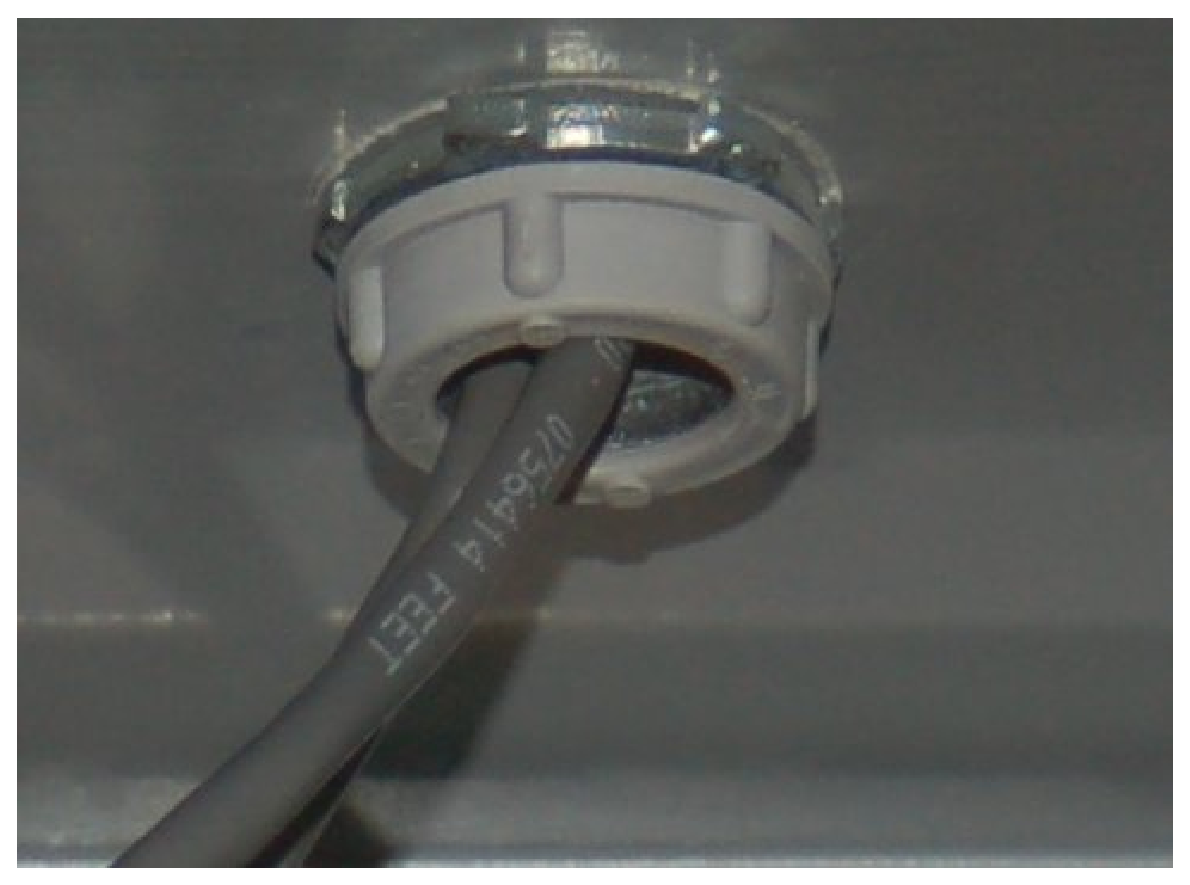
\includegraphics[width=15.5cm]{i02410x01.eps}$$

Bushings protect wires from chafing against sharp corners on the conduit connector, as the wires exit the connector and go in different directions inside an enclosure.  There are some cases where bushings may serve double-duty as wire protectors and locknuts, but their best application is purely to cover sharp edges and not to bear mechanical load.

%(END_ANSWER)





%(BEGIN_NOTES)



%INDEX% Good practices, wiring: bushings for conduit connectors

%(END_NOTES)


